% 2009 年辽宁卷理科第 18 题：两个正方形 ABCD 与 DCEF 不在同一平面内，
% M、N 分别为 AB、DF 的中点，图中连出 ME 与 BN。
% 来源 PDF：普通高考/2009/2009辽宁理.pdf，SHA256 5ae9708acfe7def5bddd60a34d1474cfa2e2c20a39d130255e0e4393093accad
% 原页：第 2 页（A3 三栏）第 1 栏上部，印刷页 538。
% 重绘依据：正方形 ABCD 竖直放置（AB 在上、CD 在下，共用边 CD），正方形 DCEF 水平展开于 CD 的
%   另一侧；M 在 AB 上、N 在 DF 上，图中连出 M 与 E、B 与 N 两条线段。原图为斜二测画法；
%   此处按同一几何关系取更清晰的斜投影，使 ME、BN 均不经过顶点 D。
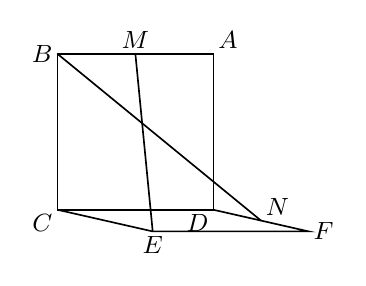
\begin{tikzpicture}[scale=1.1, semithick, every node/.style={inner sep=1.5pt, font=\small}]
  \coordinate (D) at (0,0);
  \coordinate (C) at (-1.8,0);
  \coordinate (B) at (-1.8,1.8);
  \coordinate (A) at (0,1.8);
  \coordinate (E) at (-0.7,-0.25);
  \coordinate (F) at (1.1,-0.25);
  \coordinate (M) at (-0.9,1.8);
  \coordinate (N) at (0.55,-0.125);
  % 竖直正方形 ABCD
  \draw (A) -- (B) -- (C) -- (D) -- cycle;
  % 水平正方形 DCEF
  \draw (C) -- (E) -- (F) -- (D);
  % 图中线段 ME、BN
  \draw (M) -- (E);
  \draw (B) -- (N);
  % 顶点标注
  \node[above right] at (A) {$A$};
  \node[left] at (B) {$B$};
  \node[above] at (M) {$M$};
  \node[below left] at (C) {$C$};
  \node[below left] at (D) {$D$};
  \node[below] at (E) {$E$};
  \node[right] at (F) {$F$};
  \node[above right] at (N) {$N$};
\end{tikzpicture}
